\documentclass[a4paper, 11pt, twoside]{article}
\usepackage[outer={2.5cm},inner={3cm},tmargin={2.5cm},bmargin={2cm}]{geometry}
\usepackage{amsmath}
\usepackage{amssymb}
\usepackage{amsthm}
\usepackage{hyperref}
\usepackage{colonequals}
\usepackage{xfrac}
\usepackage{tikz}
\usepackage{tikz-cd}

\usepackage{graphicx}
\usepackage{caption}

\setlength{\parindent}{0mm}
\setcounter{MaxMatrixCols}{100}

\newcommand{\R}[0]{\mathbb{R}}
\newcommand{\N}[0]{\mathbb{N}}
\newcommand{\T}[0]{\mathcal{T}}
\newcommand{\NB}[0]{\mathcal{N}}
\newcommand*{\logeq}{\ratio\Leftrightarrow}
\newcommand*{\longeq}{\ratio\Longleftrightarrow}
\newcommand*{\bigdot}{\mathpalette\bigcdot@{.5}}
\DeclareRobustCommand{\loongrightarrow}{%
  \DOTSB\relbar\joinrel\relbar\joinrel\rightarrow
}

\title{Seminar thesis - Fundamental groups as limits of discrete fundamental groups}
\author{Yannik Höll}
\date{\today}

\newtheoremstyle{break}%
{7pt}{7pt}%
{}{}%
{\bfseries}{:}% % Note that final punctuation is omitted.
{\newline}{}

\theoremstyle{break}
\newtheorem{thm}{Theorem}[section]

\theoremstyle{break}
\newtheorem{defin}[thm]{Definition}
\newtheorem{rem}[thm]{Remark}
\newtheorem{lemma}[thm]{Lemma}
\newtheorem{col}[thm]{Corollary}
\newtheorem{ex}[thm]{Example}

\begin{document}

\nocite{*}

\maketitle

\section*{Introduction}
This seminar thesis is concerned with the work of Vigolo on the study of the inverse limit of discrete first fundamental groups (\cite{vigolo2018fundamental}). The discrete version serves as an approximation
for the continuous analogue. But this approximation only makes sense if in the limit the discrete fundamental group is isomorphic to the fundamental group.

The author formulated conditions on the underlying metric space such that the discretization map is an isomorphism. 
Additionally, examples of metric spaces are presented which do not have the aforementioned properties and it is shown that the discretization map is not an isomorphism
in these spaces. This demonstrates the sharpness of the conditions.

The first chapter in this thesis establishes basic topological facts and definitions and defines the fundamental group $\pi_1(X)$ of a topological space.
Then in the second chapter the discrete version of $\pi_1(X)$ is introduced and some important properties of it are proven.
Following in the third chapter is the definition of the categorical notion of inverse limit and the application to the discrete fundamental group. 
And the thesis closes with a selection of the examples of metric spaces presented in the paper. 

\section{Basic topological definitions} \label{section-basic-defs}

The definitions and proofs provided in this chapter are common knowledge and can be looked up in standard textbooks of topology like \cite{munkres2000topology}.

\textbf{Notation:}
\begin{enumerate}
  \item Let $Y$ be a topological space with the topology $\T_Y$,
  \item Let $X$ be a metric space with the metric $d_X$ which is also a topological space with the topology induced by its metric,
  \item If $Z_1, Z_2$ are topological spaces then $C(Z_1, Z_2)$ is the set of all continuous maps from $Z_1$ to $Z_2$,
  \item Let $y \in Y$ then $\NB_y$ is the set of all neighbourhoods of the element $y$.
  \item Let $\varepsilon \in \R_{>0}$ and let $x \in X$: $B_{\varepsilon}(x) := \{ y\in X \: | \: d_X(x, y) < \varepsilon\}$
\end{enumerate}

\begin{defin}
  A \textbf{path} $\gamma$ in $Y$ is a continuous map $[0,1] \to Y$ where $[0,1]$ is seen as a subspace of $\R$.
\end{defin}

\begin{defin}
  Let $\gamma_1, \gamma_2 \in C([0, 1], Y)$. A \textbf{free homotopy} $H\colon [0,1]^2 \to Y$ between $\gamma_1$ and $\gamma_2$ is a continuous map such that:
  \begin{equation*}
    \forall s \in [0,1]\colon H(s, 0) = \gamma_1(s) \: \land \: H(s, 1) = \gamma_2(s)
  \end{equation*}

  Now let $\gamma_1, \gamma_2 \in C([0, 1], Y)$ such that $\gamma_1(0) = \gamma_2(0)$ and $\gamma_1(1) = \gamma_2(1)$ i.e. both paths start and end at the same point.
  The homotopy $H \in C([0,1]^2, Y)$ is called \textbf{endpoint preserving} if it is a free homotopy between $\gamma_1$ and $\gamma_2$ and it has the following property 
  \begin{equation*}
    \forall t\in[0,1]\forall i\in \{1,2\}: H(0, t) = \gamma_i(0) \: \land \: H(1, t) = \gamma_i(1).
  \end{equation*}

  If a free homotopy $H$ between the two paths $\gamma_1$ and $\gamma_2$ exists they are called \textbf{freely homotopic} $\gamma_1 \overset{\cdot}{\sim}_H \gamma_2$.
  If the two paths $\gamma_1$ and $\gamma_2$ have the same start and end point and there exists an endpoint preserving homotopy $H$ between them then they are called 
  \textbf{homotopic} $\gamma_1 \sim_H \gamma_2$. If a path is (freely) homotopic to a constant path ($[0,1] \to Y, t \mapsto y \in Y$) then it is called \textbf{null-homotopic}.

  Lastly define the homotopy relation $\sim$ on $C([0,1], Y)$ where 
  \begin{equation*}
    \forall\gamma_1, \gamma_2 \in C([0,1], Y)\colon \gamma_1 \sim \gamma_2 \iff \exists H \text{ homotopy between } \gamma_1 \text{ and } \gamma_2.
  \end{equation*}
\end{defin}

In this thesis all homotopies are endpoint preserving if it is not explicitly stated that they should be free homotopies.

\begin{defin} \label{def:connectedness}
  \begin{itemize}
    \item[] % this has to be here because of the newline after the definition label
    \item $Y$ \textbf{connected} $\;\longeq\; \exists A,B \in \T_Y\setminus \{\emptyset\}\colon (A \cap B = \emptyset \: \land \: Y = A \cup B) \Rightarrow (A = \emptyset \: \lor \: B = \emptyset)$
    \item $Y$ \textbf{path-connected} $\;\longeq\; \forall x,y \in Y \exists\gamma \in C([0,1], Y)\colon \gamma(0) = x \: \land \: \gamma(1) = y$
    \item $Y$ \textbf{locally (path-)connected} $\;\longeq \\ \forall y \in Y\forall U \in \NB_y\exists V\in \NB_y\colon V \subseteq U \: \land \: V$ (path-)connected
  \end{itemize}
\end{defin}

The following definitions only work in metric spaces:

\begin{defin}
  \begin{itemize}
    \item[] % this has to be here because of the newline after the definition label
    \item $X$ \textbf{uniformly locally path-connected} (u.l.p.c.) $\: \longeq \\ \forall \varepsilon \in \R_{>0} \exists \delta \in \R_{>0}\forall x \in X\colon \forall x_1, x_2 \in B_{\delta}(x)\exists \gamma \in C([0,1], B_{\varepsilon}(x))\colon \gamma(0) = x_1 \: \land \: \gamma(1) = x_2$
    \item $X$ \textbf{semi-locally simply connected} (s.l.s.c) $\: \longeq \\ \forall x\in X\exists \varepsilon \in \R_{>0}\colon$ Every loop in $B_{\varepsilon}(x)$ is null-homotopic in $X$
    \item $X$ \textbf{uniformly semi-locally simply connected} (u.s.l.s.c) $\: \longeq \\ \exists \varepsilon \in \R_{>0}\forall x\in X\colon$ Every loop in $B_{\varepsilon}(x)$ is null-homotopic in $X$
  \end{itemize}
  \vspace*{10pt}
  For clarification, the difference between semi-locally simply connectedness and uniformly semi-locally simply connected is 
  that in the first case $\varepsilon$ is chosen dependent on $x$ and in the latter case it is chosen independently for all $x$.
\end{defin}

\begin{lemma} \label{lem:homotopy-equivalence}
  The homotopy relation $\sim$ of paths is an equivalence relation on the set $C([0,1],Y)$.
\end{lemma}

\begin{proof}
  Let $\gamma_1, \gamma_2, \gamma_3 \in C([0,1],Y)$ with $\gamma_1(0) = \gamma_2(0) = \gamma_3(0)$ and $\gamma_1(1) = \gamma_2(1) = \gamma_3(1)$.
  
  \textit{Reflexivity:}
  Consider the homotopy $H\colon [0,1]^2 \to Y, \: (s, t) \mapsto \gamma_1(s)$. 
  
  It holds that for all $s\in [0,1]\colon H(s, 0) = \gamma_1(s),\: H(s, 1) = \gamma_1(s)$. And thus $\gamma_1 \sim_H \gamma_1 \Rightarrow \gamma_1 \sim \gamma_1$.

  \textit{Symmetry:} 
  Assume that $\gamma_1 \sim \gamma_2$. This means there exists a homotopy $H$ such that $\gamma_1 \sim_H \gamma_2$. 
  Now define the homotopy $F\colon [0,1]^2 \to Y, \: (s, t) \mapsto H(s, 1-t)$. 
  
  From this definition it follows that for all $s \in [0,1]:$
  \begin{align*}
    F(s, 0) &= H(s, 1 - 0) = \gamma_2(s) \\
    F(s, 1) &= H(s, 1 - 1) = \gamma_1(s)
  \end{align*}
  and hence $\gamma_2 \sim_F \gamma_1 \Rightarrow \gamma_2 \sim \gamma_1$.

  \textit{Transitivity:}
  Assume that $\gamma_1 \sim \gamma_2$ and $\gamma_2 \sim \gamma_3$. Let $H$ be a homotopy between $\gamma_1$ and $\gamma_2$ and let $F$ be a homotopy between $\gamma_2$ and $\gamma_3$. 
  Define the homotopy
  \begin{equation*} 
    G: [0,1]^2 \to Y, \: (s,t) \mapsto \begin{cases}
      H(s, 2t), &t \in [0, {1 \over 2}], \\
      F(s, 2t - 1), &t \in [{1 \over 2}, 1].
    \end{cases}
  \end{equation*}

  Then the following equations hold
  \begin{align*}
    G(s,0) &= H(s,0) = \gamma_1(s), \\
    G\left(s, \tfrac{1}{2}\right) &= H(s, 1) = \gamma_2(s) = F(s, 0), \\
    G(s, 1) &= F(s, 1) = \gamma_3(s),
  \end{align*}
  and thus $\gamma_1 \sim_G \gamma_3 \Rightarrow \gamma_1 \sim \gamma_3$.
\end{proof}

\begin{rem} \label{rem:reparam}
  Let $\alpha: [0,1] \to [0,1]$ be a continuous map with $\alpha(0) = 0, \alpha(1) = 1$ and let $\gamma \in C([0,1], Y)$. Then it follows that $\gamma \sim \gamma \circ \alpha$.
\end{rem}

\begin{proof}
  Let $F\colon [0,1]^2 \to Y, (s, t) \mapsto \gamma((1 - t)s + t\alpha(s))$.

  At first let $s \in [0,1]$ fixed and let $\alpha(s) \in [0,1]$ then $(1 - t)s + t\alpha(s)$ is a convex combination of the two points. 
  $[0,1]$ is a convex set and thus for all $t\in[0,1]$ it is true that $(1 - t)s + t\alpha(s) \in [0,1]$. Because of the continuity of the operations $+$ and $\cdot$ in $[0,1]$ 
  and the continuity of $\alpha$ the map $F$ is continuous and the following hold
  \begin{align*}
    F(s, 0) &= \gamma(s), \\
    F(s, 1) &= \gamma(\alpha(s)),
  \end{align*}
  and thus $\gamma \sim_F \gamma \circ \alpha$ which means $\gamma \sim \gamma \circ \alpha$.
\end{proof}

\begin{defin}
  Let $y_0 \in Y$. The \textbf{fundamental group} of the topological space $Y$ with base point $y_0$ is defined as follows
  \begin{equation*}
    \pi_1(Y, y_0) := (\{\gamma \in C([0,1],Y) \: | \: \gamma(0) = \gamma(1) = y_0\}/_{\sim}, \: *)
  \end{equation*}
  where 
  \begin{equation*} 
    *\colon C([0,1], Y) \times C([0,1], Y) \to C([0,1], Y), (\gamma_1, \gamma_2) \mapsto \left(t \mapsto \begin{cases}
    \gamma_1(2t),   &t \in [0, {1 \over 2}], \\
    \gamma_2(2t-1), &t \in [{1 \over 2}, 1],
  \end{cases}\right)
\end{equation*}
is the concatenation of paths. The case $t = {1\over2}$ is included in both cases because the operation is only defined for paths $\gamma_1, \gamma_2$ if $\gamma_1(1) = \gamma_2(0)$. 
In the case of the fundamental group this is fulfilled for every path because all paths are loops that start and end at the same base point.

The operation $*\colon \pi_1(Y, y_0) \times \pi_1(Y, y_0) \to \pi_1(Y, y_0)$ is defined as
\begin{equation*}
  ([\gamma_1]_{\sim}, [\gamma_2]_{\sim}) \mapsto [\gamma_1]_{\sim} * [\gamma_2]_{\sim} = [\gamma_1 * \gamma_2]_{\sim}.
\end{equation*} 
\end{defin}

\begin{thm}
  Let $y_0 \in Y$. The fundamental group $\pi_1(Y, y_0)$ is a well-defined group. 
\end{thm}

\begin{proof}
  By Lemma \ref{lem:homotopy-equivalence} $\sim$ is a well-defined equivalence relation and thus the quotient in the definition is well-defined and the set of loops based at $y_0$ is decomposed into equivalence classes.
  Thus it remains to be shown that the set of equivalence classes of loops with respect to homotopy together with the concatenation operation $*$ fulfills the group axioms.

  Therefore let $\gamma_1, \gamma_2$ be loops in $Y$ based at $y_0 \in Y$. From the definition of $*$ it is clear that $\gamma_1 * \gamma_2$ is a loop in $Y$ based at $y_0$.
  Now let $\tilde{\gamma_1}$ be another loop based at $y_0$ that is homotopic to $\gamma_1$ via the homotopy $H$. Define $F\colon [0,1]^2 \to Y$ in the following way
  \begin{equation*}
    (s, t) \mapsto \begin{cases}
      H(2s, t), &s \in [0,{1 \over 2}], \\
      \gamma_2(s), &s \in [{1 \over 2}, 1].
    \end{cases}
  \end{equation*}
  This is a well-defined homotopy between $\gamma_1 * \gamma_2$ and $\tilde{\gamma_1} * \gamma_2$ because of
  \begin{align*}
    F(s, 0) &= \gamma_1 * \gamma_2, \\
    F(s, 1) &= \tilde{\gamma_1} * \gamma_2.
  \end{align*}
  
  There is no problem for $t = {1 \over 2}$ because the homotopy is endpoint preserving. Thus it holds that $\gamma_1 \sim \tilde{\gamma_1} \Rightarrow \gamma_1 * \gamma_2 \sim \tilde{\gamma_1} * \gamma_2$.
  And a similar argument shows $\gamma_1 \sim \tilde{\gamma_1} \Rightarrow \gamma_2 * \gamma_1 \sim  \gamma_2 * \tilde{\gamma_1}$. 
  This proves that the group operation is not dependent on the choice of representative of the particular equivalence class which means that the group operation is well-defined.

  Now let $\gamma_3$ be another loop in $Y$ based at $y_0$. 

  Consider the map $\alpha\colon [0,1] \to [0,1]$ which is defined as
  \begin{equation*}
    t \mapsto \begin{cases}
      2t, &t \in [0, {1 \over 4}], \\
      t + {1 \over 4}, &t \in [{1\over4}, {1\over2}], \\
      {1\over2}t + {1\over2}, &t\in[{1\over2}, 1].
    \end{cases}
  \end{equation*}
  By definition it is true that $\alpha(0) = 0, \alpha(1) = 1$ and $((\gamma_1 * \gamma_2) * \gamma_3) \circ \alpha = \gamma_1 * (\gamma_2 * \gamma_3)$ and thus $(\gamma_1 * \gamma_2) * \gamma_3 \sim \gamma_1 * (\gamma_2 * \gamma_3)$ by Remark \ref{rem:reparam}.
  Hence the operation $*$ is associative.
  
  Next consider the constant path $e_{y_0}\colon [0,1] \to Y, \: t \mapsto y_0$ at $y_0$. 
  
  \vspace*{5pt}
  Define $\alpha_1\colon [0,1] \to [0,1], \: t \mapsto \begin{cases}
    0, &t\in[0, {1\over2}],\\
    2t, &t\in[{1\over2}, 1],
  \end{cases}$ and $\alpha_2\colon [0,1]\to [0,1], \: t \mapsto \begin{cases}
    2t, &t\in[0, {1\over2}],\\
    0, &t\in[{1\over2}, 1],
  \end{cases}$

  with $\alpha_1(0) = \alpha_2(0) = 0$ and $\alpha_1(1) = \alpha_2(1) = 1$.

  It follows for a loop $\gamma$ in $Y$ based at $y_0$ that $e_{y_0} * \gamma = \gamma \circ \alpha_1$ and $\gamma * e_{y_0} = \gamma \circ \alpha_2$ and thus by Remark \ref{rem:reparam}
  \begin{equation*}
    \gamma * e_{y_0} \sim \gamma \sim e_{y_0} * \gamma
  \end{equation*}
  This means that $e_{y_0}$ is the identity element with respect to $*$.

  Now let $\gamma^-$ be a loop in $Y$ based at $y_0$ defined by $\gamma^-(t) := \gamma(1 - t)$ for all $t \in [0,1]$ and consider the homotopy $G\colon [0,1]^2 \to Y$ with 
  \begin{equation*}
    (s, t) \mapsto \begin{cases}
      \gamma(2s(1-t)), &t \in [0, {1\over2}], \\
      \gamma(2(1-s)(1-t)), &t \in [{1\over2}, 1],
    \end{cases}
  \end{equation*}
  is a homotopy between $\gamma * \gamma^-$ and $e_{y_0}$ which means $[\gamma] * [\gamma^-] = [\gamma * \gamma^-] = [e_{y_0}]$ and thus $[\gamma^-] = [\gamma]^{-1}$. 
\end{proof}

\begin{lemma}\label{lem:lesbesgue}
  Let $\mathcal{U}$ be an open cover of $X$. If $X$ is compact, then there exists $\delta \in \R_{>0}$ such that:
  \begin{equation*}
    \forall A \in \mathcal{P}(X)\colon d(A) < \delta \Rightarrow (\exists U \in \mathcal{U}\colon A \subseteq U),
  \end{equation*}
  where $d\colon \mathcal{P}(X) \to [0, \infty), \: A \mapsto \sup \{ d_X(a_1, a_2) \: | \: a_1,a_2\in A \}$ is the diameter of a subset of $X$.
\end{lemma}

\begin{proof}
  See \cite[p. 175f.]{munkres2000topology}
\end{proof}

\section{Discretization of the fundamental group}
\textbf{Notation:}
\begin{enumerate}
  \item Let $n \in \N$: $[n] := \{0, 1, \ldots, n\}$,
  \item Let $n,m \in \N$ with $n \leq m$: $[n,m] := \{n, n+1, \ldots, m\}$.
\end{enumerate}

The notion of the fundamental group introduced in the previous chapter is very a useful tool for determining if two topological spaces are \textbf{not} homeomorphic.
The fundamental group has this ability because it is a functor from the category of topological spaces with a fixed base point to the category of groups. 
And if the images of a functor are not isomorphic then the arguments that mapped to these images can not be isomorphic in their category because functors preserve isomorphisms.

A major disadvantage of the fundamental group is that it is very computationally difficult to calculate.
That's the reason why there exist many other branches of algebraic topology concerned with other topological invariants that are invariant under homeomorphisms. 
Another fruitful idea would be to reduce the difficulty in calculating the fundamental group by approximating it via discrete fundamental groups. 
This concept is explored further in the following chapter.

\begin{defin} \label{def:discrete-path}
  Let $\theta \in \R_{>0}$ and $n \in \N$. A \textbf{discrete path} ($\theta$-path) with length $n$ is a map $Z: [n] \to X$ that is $\theta$-Lipschitz with respect to the restriction of the euclidean metric on $\R$ to $[n]$, i.e.
  \begin{equation}
    \forall n_1, n_2 \in [n]\colon d_X(Z(n_2), Z(n_1)) \leq \theta |n_2 - n_1|.
  \end{equation}
  An important special case is $n_2 = n_1 + 1$ for $n_1, n_2 \in [n]$ for which holds: $d_X(Z(n_1), Z(n_2)) \leq \theta$. This motivates a second
  definition of a discrete path as a sequence of points $(z_i)_{i=0}^n$ with $z_i \in X$ and
  \begin{equation}
    \forall i \in \{0, 1, \ldots, n-1\} \colon d_X(z_i, z_{i+1}) \leq \theta.
  \end{equation}

  Let $m \in \N$ with $m \geq n$ and let $Z'\colon [m] \to X$ be a discrete path. $Z'$ is called a \textbf{lazification} of $Z$ if there exists a surjective, monotone map 
  $f\colon [m] \to [n]$ such that $Z' = Z \circ f$. 
  
  \cite[p. 3]{vigolo2018fundamental}
\end{defin}

\begin{defin}
  Let $\theta \in \R_{>0}$, $n,m \in \N$ and let $Z_1\colon [n] \to X, Z_2: [n] \to X$ be two discrete $\theta$-paths in $X$. 
  A \textbf{(free) $\theta$-grid homotopy} is a $\theta$-Lipschitz map $H\colon [n] \times [m] \to X$ such that
  \begin{equation*}
    H(\cdot, 0) = Z_1 \: \land \: H(\cdot, m) = Z_2,
  \end{equation*}
  where the product $[n] \times [m]$ is a metric space with the $\ell_1$ metric\footnote{i.e. for $x = (x_1, x_2), y = (y_1, y_2) \in [n] \times [m]\colon d_{\ell_1}(x, y) = |x_1 - y_1| + |x_2 - y_2|$}.

  A free $\theta$-grid homotopy is a $\theta$-grid homotopy if it preserves the endpoints of the discrete paths i.e.
  \begin{equation*}
    \forall t\in [m]\colon H(0,t) = Z_1(0) = Z_2(0) \: \land \: H(n,t) = Z_1(n) = Z_2(n),
  \end{equation*}
  for paths $Z_1, Z_2$ with the same start and end points.

  \cite[p. 3]{vigolo2018fundamental}
\end{defin}

% source BCW14
\begin{rem}
  Let $(x_0, x_1, \ldots, x_n)$ and $(y_0, y_1, \ldots, y_n)$ with $n \in \N, y_0 = y_n$ and $x_0 = x_n$ be two closed $\theta$-paths in $X$. 
  One can imagine a $\theta$-grid homotopy as a grid
  \begin{equation*}
    \begin{matrix}
      x_0 & x_1 & x_2 & \cdots & x_n \\
      z_0^1 & z_1^1 & z_2^1 & \cdots & z_n^1 \\
      \vdots & \vdots & \vdots & \vdots & \vdots \\
      z_0^{t} & z_1^{t} & z_2^{t} & \cdots & z_n^{t} \\
      y_0 & y_1 & y_2 & \cdots & y_n \\
    \end{matrix}
  \end{equation*}
  where the rows are $\theta$-loops in $X$ and the columns are $\theta$-paths in $X$ and $t\in \N$.

  \cite[p. 3, Def. 2.2]{barcelo2014discrete}
\end{rem}

\begin{defin}
  Let $\theta \in \R_{>0}$ and let $Z_1, Z_2$ be discrete $\theta$-paths. $Z_1$ and $Z_2$ are said to be $\theta$-homotopic 
  if there exist lazifications $Z_1'$ of $Z_1$ and $Z_2'$ of $Z_2$ with the same length and a $\theta$-grid homotopy between $Z_1'$ and $Z_2'$.
  
  This is denoted as $Z_1 \sim_{\theta} Z_2$.

  \cite[p. 3, Def. 2.2]{vigolo2018fundamental}
\end{defin}

\begin{defin}
  Let $\theta \in \R_{>0}$ and $x_0 \in X$. $\mathcal{C}_{\theta}(X, x_0)$ is the set of all discrete closed $\theta$-paths in $X$ starting and ending at $x_0$. Now take $x, y \in \mathcal{C}_{\theta}(X, x_0)$.
  
  By the Definition \ref{def:discrete-path} there are $m,n \in \N$ such that we can write
  \begin{equation*}
    x = (x_0, x_1, \ldots, x_n = x_0), \: y = (y_0, y_1, \ldots, y_m = y_0)
  \end{equation*} where for all $i \in [n]\colon x_i \in X$ and for all $j \in [m]: y_j \in X$.

  Now define the concatenation of paths $*\colon \mathcal{C}_{\theta}(X, x_0) \times \mathcal{C}_{\theta}(X, x_0) \to \mathcal{C}_{\theta}(X, x_0), (x, y) \to x * y$ where
  \begin{equation*}
    x * y = (x_0, x_1, \ldots, x_n = y_0, y_1, \ldots, y_m)
  \end{equation*}
  i.e. $x * y\colon [n+m] \to X, t \mapsto \begin{cases}
    x_t, &t \in [n], \\
    y_{t-n}, &t \in [n,n+m].
  \end{cases}$

  \cite[p. 3]{barcelo2014discrete}
\end{defin}

\begin{lemma} \label{lem:discrete-homotopy}
  Let $\theta \in \R_{>0}$ then the $\theta$-grid homotopy relation $\sim_{\theta}$ on the set $\mathcal{C}_{\theta}(X, x_0)$ is an equivalence relation.
\end{lemma}

\begin{proof}
  Similar to proof of \ref{lem:homotopy-equivalence}.
\end{proof}

\begin{defin}
  Let $\theta \in \R_{>0}$ and let $x_0 \in X$. $\pi_{1,\theta}(X, x_0) := (\mathcal{C}_{\theta}(X, x_0)/_{\sim_{\theta}}, *)$ is called the \textbf{discrete fundamental group} at scale $\theta$,
  with $*\colon \pi_{1,\theta}(X, x_0) \times \pi_{1,\theta}(X, x_0) \to \pi_{1,\theta}(X, x_0), ([x]_{\theta}, [y]_{\theta}) \mapsto [x * y]_{\theta}$.
\end{defin}

\begin{thm}
  Let $\theta \in \R_{>0}$ and $x_0 \in X$. The discrete fundamental group $\pi_{1,\theta}(X, x_0)$ is a well-defined group.
\end{thm}

\begin{proof}
  Firstly the set $\mathcal{C}_{\theta}(X, x_0)/_{\sim_{\theta}}$ is well-defined because of Lemma \ref{lem:discrete-homotopy}.

  Now let $[x]_{\theta}, [y]_{\theta} \in \pi_{1, \theta}(X, x_0)$. Let $x, \tilde{x} \in [x]_{\theta}$ and $y \in [y]_{\theta}$.
  Then there exist lazifications $x', \tilde{x}'$ of $x, \tilde{x}$ and $y'$ of $y$ with the same length $m \in \N$ 
  and a $\theta$-grid homotopy $H\colon [n] \times [m] \to X$ with between $x'$ and $\tilde{x}'$ ($n \in \N$).

  Let $k \in \N$ and define the map $\tilde{H}\colon [n] \times [2m] \to X$ as follows
  \begin{equation*}
    \tilde{H}(s, t) = \begin{cases}
       H(s, t), &t \in [m], \\
       y'(t-m), &t \in [m,2m].
    \end{cases}
  \end{equation*}
  Since the maps $H$ and $y'$ are $\theta$-Lipschitz and for all $s \in [n]$ it is true that $x_0 = H(s,m) = y(0)$ 
  it follows from the pasting Lemma for $\theta$-Lipschitz maps (\cite[Thm. 1]{kvalheim2021pasting}) that $\tilde{H}$ is $\theta$-Lipschitz.
  Since for all $t \in [2m]$ it holds that $\tilde{H}(0, t) = (x' * y')(t)$ and $\tilde{H}(n, t) = (\tilde{x}' * y')(t)$,
  $x * y \sim_{\theta} \tilde{x} * y$ follows and thus $[x * y]_{\theta} = [\tilde{x} * y]_\theta$.

  A similar argument can be used to proof the claim for the right side of $*$. 
  
  It follows that $[x * y]_{\theta} = [\tilde{x} * \tilde{y}]_{\theta}$ if $\tilde{y} \in [y]_\theta$ 
  which means that the group operation is independent from the choice of representative.

  \textit{Associativity:}
    Let $[x]_{\theta}, [y]_{\theta}, [z]_{\theta} \in \pi_{1,\theta}(X, x_0)$ 
    and let $x', y', z'$ be lazifications of the discrete paths with length $m$ which is the maximum of the lengths of $x,y,z$. Consider:
    \begin{align*}
      f(t) := (x' * y') * z' &= \begin{cases}
        (x' * y')(t), &t \in [2m], \\
        z'(t - 2m), &t \in [2m, 3m],
      \end{cases}\\
      g(t) := x' * (y' * z') &= \begin{cases}
        x'(t), &t \in [m], \\
        (y' * z')(t - m), &t \in [m, 3m],
      \end{cases}
    \end{align*}
  \begin{enumerate}
    \item $t \in [m]\colon f(t) = (x' * y')(t) = x'(t) = g(t)$,
    \item $t \in [m,2m]\colon f(t) = (x' * y')(t) = y'(t - m) = (y' * z')(t - m) = g(t)$,
    \item $t \in [2m,3m]\colon f(t) = z'(t - 2m) = (y' * z')(t - m) = g(t)$,
  \end{enumerate}
  and thus $f = g\:$ i.e. $[x]_{\theta} * ([y]_{\theta} * [z]_{\theta}) = [x * (y * z)]_{\theta} = [(x * y) * z]_{\theta} = ([x]_{\theta} * [y]_{\theta}) * [z]_{\theta}$.
  
  \textit{Identity:}
  Let $e_{x_0}\colon [0] \to X, 0 \mapsto x_0$ be the constant path at $x_0$. Then $x * e_{x_0} = x'$ and $e_{x_0} * x = x''$ with $x'$ and $x''$ lazifications of $x$ 
  and hence $e_{x_0} * x \sim_{\theta} x \sim_{\theta} x * e_{x_0}$.
  It follows that $[x]_{\theta} * [e_{x_0}]_{\theta} = [x * e_{x_0}]_{\theta} = [x]_{\theta}$ and $[e_{x_0}]_{\theta} * [x]_{\theta} = [e_{x_0} * x]_{\theta} = [x]_{\theta}$.
  
  \textit{Inverse:}
  Let $x \in \mathcal{C}_{\theta}(X, x_0)$ with length $m$. Define the path $x^-\colon [m] \to X, t \mapsto x(m - t)$ where $n$ is the length of $x$.

  Define $H\colon [m] \times [2m] \to X$ given by the following schema
  \begin{equation*}
    \begin{matrix}
      x_0 & x_1 & x_2 & \cdots & x_{m-2} & x_{m-1} & x_m = x_0 & x_{m-1} & x_{m-2} & \cdots & x_1 & x_0 \\
      x_0 & x_1 & x_2 & \cdots & x_{m-2} & x_{m-1} & x_{m-1} & x_{m-1} & x_{m-2} & \cdots & x_1 & x_0 \\
      x_0 & x_1 & x_2 & \cdots & x_{m-2} & x_{m-2} & x_{m-2} & x_{m-2} & x_{m-2} & \cdots & x_1 & x_0 \\
      \vdots & \vdots & \vdots & \vdots & \vdots & \vdots & \vdots & \vdots & \vdots & \vdots & \vdots & \vdots \\
      x_0 & x_0 & x_0 & \cdots & x_0 & x_0 & x_0 & x_0 & x_0 & \cdots & x_0 & x_0 \\
    \end{matrix}
  \end{equation*}
  The $n$th row contains the path $x$ up to $t = m-n$, continuing with $2n-1$ copies of $x_{m-n}$ and ending with $x_{m-n}$ up to $x_0$.
  It is trivial to show that each row is a correct $\theta$-loop. It remains to show that each column is a $\theta$-path. To this end let $i \in [m]$ and define the $i$th row as $r\colon [m] \to X$.
  Then by construction if $t \in [m-i]$ then $r(t) = x_t$ and if $t \in [m-i+1, m]$ then $r(t) = x_{m-(t-i)}$. 
  Now it follows that $d_X(r(i), r(i+1)) \leq \theta$ and hence $r$ is a $\theta$-path.
\end{proof}

\begin{rem}
  For $\theta' \leq \theta$ there exists a natural homomorphism $\pi_{1,\theta'}(X, x_0) \to \pi_{1,\theta}(X, x_0)$ 
  because every $\theta'$-path is also a $\theta$-path and every $\theta'$-grid homotopy is also a $\theta$-grid homotopy.
\end{rem}

\begin{rem}
  Every closed $\theta$-path with length $\leq 4\theta$ is $\theta$-homotopic to a constant path.

  \cite[p. 4]{vigolo2018fundamental}
\end{rem}

\begin{proof}
  Consider a closed $\theta$-path $(z_0, z_1, z_2, z_3, z_4 = z_0)$ in $X$. 
  Define the constant path $e_{z_0}\colon [0] \to X, 0 \mapsto z_0$ and the lazification $Z': [4] \to X, i \mapsto z_0$ of $Z$.

  Then $(z_0, z_1, z_2, z_3, z_4 = z_0) \sim_{\theta} (z_0, z_1, z_1, z_0, z_0)\sim_{\theta} (z_0, z_0, z_0, z_0, z_0) = Z'$. The remark follows from the fact that $\sim_{\theta}$ is an equivalence relation.
\end{proof}

In this sense one can imagine that $\pi_{1,\theta}$ is isomorphic to a factor of $\pi_1$ where loops shorter than $4\theta$ are all in the equivalence class of the constant loop.

\section{Inverse Limit}

The following definition of the inverse limit is the special case in the category of groups. 
But keep in mind that this notion can be generalized to arbitrary categories.
% maybe add inverse system definition
\begin{defin}
  Let $(I, \leq)$ be a directed poset\footnote{Directed partially ordered set}, 
  $(G_i)_{i\in I}$ be a family of groups and let $(\varphi_{ij})_{i,j \in I, i \leq j}$ be a family of group homomorphisms $\varphi_{ij}\colon G_j \to G_i$ such that for all $i,j,k \in I$ with $i \leq j \leq k$
  \begin{equation*}
    \varphi_{ii} = \text{id}_{G_i} \: \land \: \varphi_{ij} \circ \varphi_{jk} = \varphi_{ik}.
  \end{equation*}
  Then the \textbf{inverse limit} of the family $(G_i)_{i\in I}$ with respect to the homomorphisms $(\varphi_{ij})_{i,j \in I, i \leq j}$ is defined as
  \begin{equation*}
    \varprojlim_{i\in I} G_i := \left\{(g_i)_{i\in I} \in \prod_{i\in I} G_i \: \middle| \: \forall i,j \in I, i \leq j: \varphi_{ij}(g_j) = g_i\right\}
  \end{equation*}
  with the group operation $(g_i)_{i\in I}, (h_i)_{i\in I} \mapsto (g_i \cdot h_i)_{i\in I}$.
\end{defin}

The construction of such inverse limits is very useful because it has the following \textit{universal property}:
\begin{figure}[ht!]
  \centering
  % https://tikzcd.yichuanshen.de/#N4Igdg9gJgpgziAXAbVABwnAlgFyxMJZAJgBoAGAXVJADcBDAGwFcYkQAJEAX1PU1z5CKMsWp0mrdgB1pDAE5p5EAFaMsAWwD6wLLKxgABAEluhgOJasPPiAzY8BIuVIBmcQxZtEISypv8DkJEACxuHpLevlY84jBQAObwRKAAZsoaSC4gOBBIAIw0nlI+smjYIDSM9ABGMIwACgKOwiAG2LABIOkQmYjZuUhkEl4y0uVYWv5VtfVNQU4+7VidvGkZWTSDiK5FkWMTMTN1jc3BS2AdbGvdG4iFOXmIw8VRZZPTINUn84KLbZcVtdbD0+g9trsRiUQO8jl9ZqcFq1lqsQXdhhC9qNSnJ6IoABaTXQqbiVeE-M7-FHXSjcIA
  \begin{tikzcd}
    &  & H \arrow[dd, dashed, "\exists!\psi" description] \arrow[llddd, "\psi_j" description] \arrow[rrddd, "\psi_i" description] &  &     \\
    &  &                                                                                                          &  &     \\
    &  & \varprojlim_{i\in I} G_i \arrow[lld, "\pi_j" description] \arrow[rrd, "\pi_i" description]               &  &     \\
  G_j \arrow[rrrr, "\varphi_{ij}" description] &  &                                                                                                          &  & G_i
  \end{tikzcd}
  \caption{Universal property of the inverse limit}\label{fig:inverse-limit}
\end{figure}

\begin{defin}
  Let $(I, \leq)$ be a directed poset, $(G_i)_{i\in I}$ be a family of groups and let $(\varphi_{ij})_{i,j \in I, i \leq j}$ be a family of group homomorphisms $\varphi_{ij} \colon G_j \to G_i$.
  Additionally, let $\pi_i$ be the projection maps from the direct product to the $i$th component.
  
  Then the inverse limit $\varprojlim_{i\in I} G_i$ has the following universal property:
  If there exists a group $H$ and a family of group homomorphisms $(\psi_i)_{i\in I}\colon H \to G_i$ such that 
  \begin{equation*}
    \forall i,j \in I\colon i \leq j \Rightarrow \varphi_{ij} \circ \psi_j = \psi_i,
  \end{equation*}
  then there exists a unique group homomorphism $\psi\colon H \to \varprojlim_{i\in I} G_i$ with the property
  \begin{equation*}
    \forall i \in I\colon \pi_i \circ \psi = \psi_i.
  \end{equation*}
  The commutative diagram in Figure \ref{fig:inverse-limit} illustrates this property.
\end{defin}

In order to use this useful property of the inverse limit we need to define maps from $\pi_1$ to $\pi_{1,\theta}$ for all $\theta \in (0,\infty)$. 
\begin{defin}
  Let $\theta \in \R_{>0}$, $\gamma\colon [0,1] \to X$ be a continuous path in $X$ and let $0 = t_0 \leq t_1 \leq \ldots \leq t_n = 1$ for $n \in \N$.

  The sequence $(\gamma(t_i))_{i=0}^n$ is called a \textbf{$\theta$-discretization} of $\gamma$ if for all $i \in \{1, \ldots, n\}$ it holds that
  \begin{equation*}
    d_X(\gamma(t_{i}), \gamma(t_{i-1})) \leq \theta.
  \end{equation*}
  The discretization of $\gamma$ is denoted as $\widehat{\gamma}^{\theta}_{(t_0, \ldots, t_n)}$.
\end{defin}

This definition is only useful if the following lemma can be proven.

\begin{lemma}\label{lem:discretization}
  Every continuous path admits a unique $\theta$-discretization up to $\theta$-homotopy. If the paths $\alpha, \beta\colon [0,1] \to X$ are homotopic then any two $\theta$-discretizations 
  $\widehat{\alpha}^{\theta}_{(t_0, \ldots, t_n)}$, $\widehat{\beta}^{\theta}_{(t_0', \ldots, t_m')}$ are $\theta$-homotopic ($n,m \in \N$).
\end{lemma}

\begin{proof}
  Let $\theta \in (0, \infty)$, $\gamma\colon [0,1] \to X$ be a continuous path in $X$. 
  
  Let $\mathcal{U} = \left\{\gamma^{-1}\left(B(x,\tfrac{\theta}{2})\right) \: \middle| \: x \in X \right\}$ which is an open cover of $[0,1]$.
  By Lemma \ref{lem:lesbesgue} there exists a $N \in \N$ such that for every $t$ in $[0,1]$ the interval $[t-1/N, t+1/N]$ is contained inside of an element of $\mathcal{U}$.
  Now set $t_i := i/N$ with $i \in \{0, \ldots, N\}$. It follows that
  \begin{equation*}
    \forall i \in \{1, \ldots, N\}\exists U \in \mathcal{U}\colon \gamma(t_{i-1}), \gamma(t_i) \in U \Rightarrow \: d_X(\gamma(t_{i-1}), \gamma(t_i)) \leq \sup\limits_{x,y \in U} d_X(x,y) = \theta,
  \end{equation*}
  which means that $\widehat{\gamma}^{\theta}_{(t_0, \ldots, t_N)}$ is a $\theta$-discretization of $\gamma$.

  Now let $n,m \in \N$ and let $\widehat{\gamma}_{(t_0, \ldots, t_n)}^{\theta}$ and $\widehat{\gamma}_{(t_0', \ldots, t_m')}^{\theta}$ be two $\theta$-discretizations of $\gamma$.
  W.l.o.g. it can be assumed that the inequalities $t_0 < t_1 < \cdots < t_n$ are all strict, $n \leq m$ and that for every $t_i$ there exists a $j \geq i$ such that $t_i = t_j'$.
  Now define the surjective, monotone map $f\colon [m] \to [n], j \mapsto \max \{t_i \leq t_j'\}$ 
  and thus $(\gamma(t_{f(0)}), \ldots, \gamma(t_{f(m)}))$ is a lazification of $(\gamma(t_0), \ldots, \gamma(t_n))$ and is $\theta$ homotopic to $(\gamma(t_0'), \ldots, \gamma(t_m'))$.
  
  Let $H\colon [0,1] \times [0,1] \to X$ be a homotopy between $\alpha$ and $\beta$. As above, Lebesgue number Lemma can be used to find a $N \in \N$ 
  such that for every pair $(t,s) \in [0,1]^2$, such that $H(B((t,s),1/N)) \subseteq B(x, \theta/2)$.
  Define $\widehat{H}^{\theta}\colon [N]^2 \to X, (i,j) \mapsto H(i/N, j/N)$. It is easy to see that $\widehat{H}^{\theta}(\cdot, 0)$ is a $\theta$-discretization of $\alpha$ and
  $\widehat{H}^{\theta}(\cdot, N)$ is a $\theta$-discretization of $\beta$ by the argument above and $\widehat{H}^{\theta}(0, \cdot)$ is a (free) $\theta$-discretization between them because by definition it holds that
  \begin{equation*}
    d_X(\widehat{H}^{\theta}(i,j), \widehat{H}^{\theta}(i,j+1)) \leq \theta, d_X(\widehat{H}^{\theta}(i,j), \widehat{H}^{\theta}(i+1,j)) \leq \theta
  \end{equation*}
  for all $i, j \in [N-1]$.

  \cite[p. 4]{vigolo2018fundamental}
\end{proof}

By Lemma \ref{lem:discretization} it follows that the discretization map $\gamma \mapsto \widehat{\gamma}^{\theta}$ is well-defined on the level of paths
and that it induces a map from $\pi_1(X, x_0)$ to $\pi_{1,\theta}(X, x_0)$ because it is easy to see that the map is compatible with the operation of path concatenation.
Furthermore, for $\theta' \leq \theta$ the diagram in Figure \ref{fig:discretization} commutes.

\begin{figure}[ht!]
  \centering
  \begin{tikzcd}
      &  & {\pi_1(X,x_0)} \arrow[lldd, "\widehat{\cdotp}^{\hspace*{1px}\theta'}" description, shift right] \arrow[rrdd, "\widehat{\cdot}^{\hspace*{1px}\theta}" description] &  &                          \\
      &  &                                                                                                                                        &  &                          \\
    {\pi_{1, \theta'}(X,x_0)} \arrow[rrrr] &  &                                                                                                                                        &  & {\pi_{1,\theta}(X, x_0)}
  \end{tikzcd}
  \caption{Discretization map}\label{fig:discretization}
\end{figure}

Now by the universal property of the inverse limit it follows that there exists a unique group homomorphism $\: \widehat{\cdot} : \pi_{1,\theta}(X, x_0) \to \varprojlim \pi_{1,\theta}(X, x_0)$.

\begin{thm} \label{thm:isomorphism}
  If $X$ is u.l.p.c. and u.s.l.s.c. then the discretization map $\: \widehat{\cdot} : \pi_{1,\theta}(X, x_0) \to \varprojlim \pi_{1,\theta}(X, x_0)$ is a group isomorphism.
\end{thm}

\begin{proof}
  Let $X$ be u.l.p.c. and u.s.l.s.c.

  \textit{Injectivity:} Since $\widehat{\cdot}\hspace*{2px}$ is a homomorphism of groups it suffices to show that the kernel is trivial.
  Since $X$ is u.s.l.s.c. there exists $\varepsilon \in \R_{>0}$ 
  such that every closed loop in $X$ with image contained in $B(x, \varepsilon)$ ($x\in X$) is null-homotopic in $X$. Furthermore,
  there exists $\delta \in (0, \varepsilon/2]$ such that for every $x \in X$ and every pair of points $a,b \in B(x, \delta)$ there is a path with image in $B(x, \varepsilon)$ connecting $a$ and $b$.
  Now let $\theta \in (0, \delta)$ and let $[\gamma] \in {\rm Ker} \hspace*{2px} \widehat{\cdot}\hspace*{2px}$. 
  This means that there exists a $\theta$-discretization $\widehat{\gamma}^{\theta}$ of $\gamma$ which is $\theta$-homotopic to the constant loop at $x_0$.
  Injectivity follows if $\gamma$ is null-homotopic in $X$.
  
  By definition there exists a grid homotopy $H\colon [n] \times [m] \to X$ ($n,m\in\N$) between $\widehat{\gamma}^{\theta}$ and the constant loop at $x_0$.
  Since $\theta < \delta$ it follows that 
  \begin{equation*}
    \forall i \in [n-1], j \in [m]\colon d_X(H(i,j), H(i+1,j)) < \delta
  \end{equation*}
  which implies the existence of a path $\alpha_{i,j}$ connecting $H(i,j)$ and $H(i+1,j)$ and
  the image of $\alpha_{i,j}$ is contained in $B(H(i,j), \varepsilon)$.
  By the same reasoning there exists a path $\beta_{i,j}$ connecting $H(i,j)$ and $H(i,j+1)$ for all $i \in [n], j \in [m-1]$ with image in $B(H(i,j), \varepsilon)$.

  Now it is possible to define a path $\xi_{i,j}$ starting at $x_0$ and ending at $H(i,j)$ by concatenation
  \begin{equation*}
    \xi_{ij} := \beta_{0,0} * \cdots * \beta_{0,j-1} * \alpha_{0,j} * \cdots * \alpha_{i-1,j}
  \end{equation*}
  for all $i \in [n], j \in [m]$ with $(i,j) \neq (0,0)$ and simply the constant path for $i = 0, j = 0$. 
  
  Now define the closed loops $\eta_{i,j}$ as
  \begin{equation*}
    \eta_{i,j} := \xi_{i,j} * \alpha_{i,j} * \beta_{i+1,j} * \alpha^{-1}_{i,j+1} * \beta^{-1}_{i,j} * \xi^{-1}_{i,j}
  \end{equation*}
  for all $i \in [n-1], j \in [m-1]$.
  The constructed loops are all null-homotopic in $X$ and the curve $\gamma$ lies inside of them. 
  This means that there exists a homotopy between $\gamma$ and the concatenation of the loops $\eta_{ij}$ that enclose $\gamma$ (when the correct order of concatenation is chosen).
  Thus $\gamma$ is null-homotopic in $X$ and $[\gamma] = [e_{x_0}]$ in $\pi_1(X, x_0)$.

  \textit{Surjectivity}: Let $(Z_{\theta})_{\theta > 0} \in \left(\left[Z_{\theta}\right]\right)_{\theta > 0} \in \varprojlim \pi_{1,\theta}(X, x_0)$. 
  Since $X$ is u.l.p.c. for every $\theta > 0$ there exists a $\delta(\theta) > 0$ such that any two points in $B(x, \delta(\theta))$ can be joined by a path with image in $B(x, \theta)$.
  Here $\delta(\theta)$ is considered to be a function of $\theta$ which is decreasing, i.e. $\delta(\theta) \geq \delta(\theta')$ for $\theta \leq \theta'$.

  Considering the path $Z_{\delta(\theta)}$. Its adjacent points can be joined by continuous paths and concatenating them in order 
  yields a closed loop $\gamma_{\theta}$ in $X$ based at $x_0$.
  $Z_{\delta(\theta)}$ is a $\theta$-discretization of $\gamma_{\theta}$.
  From the proof of the injectivity of $\; \widehat{\cdot} \;$ it follows that there exists a $\bar{\theta} > 0$ and small enough such that 
  $\: \widehat{\cdot}^{\hspace*{2px}\bar{\theta}}$ is injective. For $0 < \theta < \bar{\theta}$ is holds that:
  \begin{equation*}
    \widehat{\gamma}_{\theta}^{\theta} \sim_{\theta} Z_{\delta(\theta)} \sim_{\delta(\bar{\theta})} Z_{\delta(\bar{\theta})} \sim_{\bar{\theta}} \widehat{\gamma}_{\bar{\theta}}^{{\bar{\theta}}}
  \end{equation*}
  and thus $\widehat{\gamma}_{\theta}^{\theta}$ is $\bar{\theta}$-homotopic to $\widehat{\gamma}_{\bar{\theta}}^{{\bar{\theta}}}$ which means that
  $\gamma_{\theta} \sim \gamma_{\bar{\theta}}$.

  It can be concluded that
  \begin{equation*}
    \widehat{\gamma}_{\bar{\theta}}^{\theta} \sim_{\theta} \widehat{\gamma}_{\theta}^{\theta} \sim_{\theta} Z_{\delta(\theta)} \sim_{\theta} Z_{\theta}
  \end{equation*}
  for every $0 < \theta < \bar{\theta}$ and thus $\widehat{\gamma}_{\bar{\theta}} = \left(\left[Z_{\theta}\right]\right)_{\theta > 0} \in \varprojlim \pi_{1,\theta}(X, x_0)$.
\end{proof}

\begin{col}
  If $X$ is locally path connected, semi-locally simply connected and compact then the discretization map 
  \begin{equation*}
     \hspace*{2px}\widehat{\cdot}\hspace*{2px}\colon \pi_1(X, x_0) \to \varprojlim \pi_{1,\theta}(X, x_0)
  \end{equation*}
  is an isomorphism.
\end{col}

\begin{proof}
  It can be shown, that every locally path connected and semi-locally simply connected metric space that is compact is also u.l.p.c. and u.s.l.s.c. \cite[Lemma 5.14.4]{sakai2013geometric} The claim follows from theorem \ref{thm:isomorphism}.
\end{proof}

\section{Counterexamples}

This last chapter will present a selection of counterexamples for metric spaces which does not have all the assumptions made in theorem \ref{thm:isomorphism}.
It will be shown that regardless which assumption about $X$ (l.p.c., s.l.s.c., compactness) is dropped, 
there will be examples of metric spaces in which the map $\hspace*{2px}\widehat{\cdot}\hspace*{2px}$ is not surjective or injective.
This demonstrates that the assumptions on $X$ cannot be relaxed.

But at first, it should be mentioned that there are examples of metric spaces, where theorem \ref{thm:isomorphism} 
can be applied but there is no $\theta$ small enough such that the discretization map becomes injective or surjective.
These examples show that really only the "limit object" is isomorphic to the fundamental group and not one of the groups in the direct product.

The original work contains a counter example for every assumption and shows that the map then is either not injective or surjective. 
In the following the simplest examples will be presented and be explained in a little bit more detail. It is possible to look up the rest of the examples in \cite[p. 8ff]{vigolo2018fundamental}. 

% Select one example for surjectivity
\begin{ex}
  Consider the graph of the function $f\colon (0, 1] \to \R, \: x \mapsto \sin(1/x)$ as a subset of $\R^2$. 
  The metric space $X$ in this example is the mentioned graph union the segment $I = \{0\} \times [-1, 1]$ and union a path which joins $(1, {\rm sin}(1))$ with $(0, 0)$ 
  which does not intersect the graph nor $I$.
  $X$ is compact and simply connected, but not locally path connected.
  One can show that $\varprojlim \pi_{1,\theta}(X, 0) = \mathbb{Z}$ which means that the discretization map is not surjective.

  Intuitively speaking, this topological space is like a very distorted version of the unit circle. 
  Nevertheless, $\pi_1(X)$ is trivial because there is no continuous path enclosing the "hole" in this topological space because it is not locally path connected.
  
  The discrete versions of the fundamental group can avoid this problem because they can jump over the problematic region near the y-axis und so there are discrete paths for all 
  $\theta > 0$ enclosing the "hole".
  
  \begin{figure}[ht!]
    \centering
    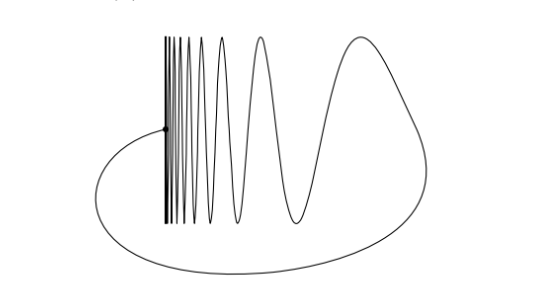
\includegraphics[width=0.5\textwidth]{ex1.png}
    \caption{The topological space $X$ \\ Source: \cite[p. 8]{vigolo2018fundamental}}
  \end{figure}
\end{ex}

\begin{ex}
  Let $X := \R^2 \setminus \{0\}$. This space is not compact. The fundamental group of this space is isomorphic to $\mathbb{Z}$. 
  But consider $\theta > 0$, then $\pi_{1,\theta}(X) = \{0\}$ which means that the discretization map cannot be injective.

  Here the "hole" in the space is infinitesimally small. The continuous fundamental group can detect it without a problem. 
  But for every $\theta > 0$ a discretization of the convex combination of two continuous paths is enough to get a $\theta$-homotopy between the 
  $\theta$-discretizations of the paths.
  It may be the case that a point of the chosen discrete homotopy lines up with the origin.
  In this case the point can be replaced with two other points near the origin which keep the $\theta$-homotopy $\theta$-Lipschitz.  
\end{ex}

\clearpage
\bibliographystyle{alpha}
\bibliography{ref} % see references.bib for bibliography management

\end{document}